\chapter{Technisch onderzoek}

\section{Voorbereiding}

Het technisch onderzoek startte bij het lezen van 'The book' een boek over de taal Rust geschreven
door Steve Klabnik, Carol Nichols en met contributies van de Rust community. Tijdens het lezen waren
er kleine code voorbeelden die u kon mee volgen. Dit maakte het makkelijker om de geavanceerde
hoofdstukken goed te begrijpen. 

Na een paar hoofdstukken diep in het boek was het tijd om de geleerde zaken tot de test te brengen.
De opdracht was om de miniversie van het gekende Linux commando grep te maken. Zo werd de geleerde
kennis over structs, ownership, enums en pattern matching, error handling, lifetimes en tests
praktisch toegepast.  

Op het einde van het boek was er een finaal project dat ook de laatste hoofdstukken bevatte. Het
project was het bouwen van een 'simpele' multi-threaded server. Daar lag de focus op het werken met
meerdere threads, wat niet voor de hand ligt als u rekening moet houden met het geheugen. 

Na de taal onder de knie te hebben, werd er onderzoek gedaan naar WebAssembly. Mits het nog een
piepjonge technologie is, was er al heel wat documentatie/artikelen over te vinden op het web. Zo
begon het onderzoek bij de documentatie van Mozilla. Daar is alles te vinden om van start te gaan
met WebAssembly. Er zijn ook doorverwijzingen naar hun uitstekende geschreven blogposts die dieper
gaan op hoe WebAssembly precies werkt.

Vervolgens moest er een keuze gemaakt worden welke frameworks we zullen gebruiken voor het bouwen
van de webapplicatie. Na wat onderzoek dat beschreven staat in \enquote{Welke front- end backend
frameworks zijn er ter beschikking?}, is er gekozen voor Yew als frontend en Actix web samen met
diesel.rs als backend frameworks.

\clearpage

\section{Omschrijving}

Om de huidige status van Rust voor het bouwen van webapplicaties te onderzoeken, werd er gekozen
voor een speed typing test applicatie te maken.

\begin{figure}[h]
  \centering
  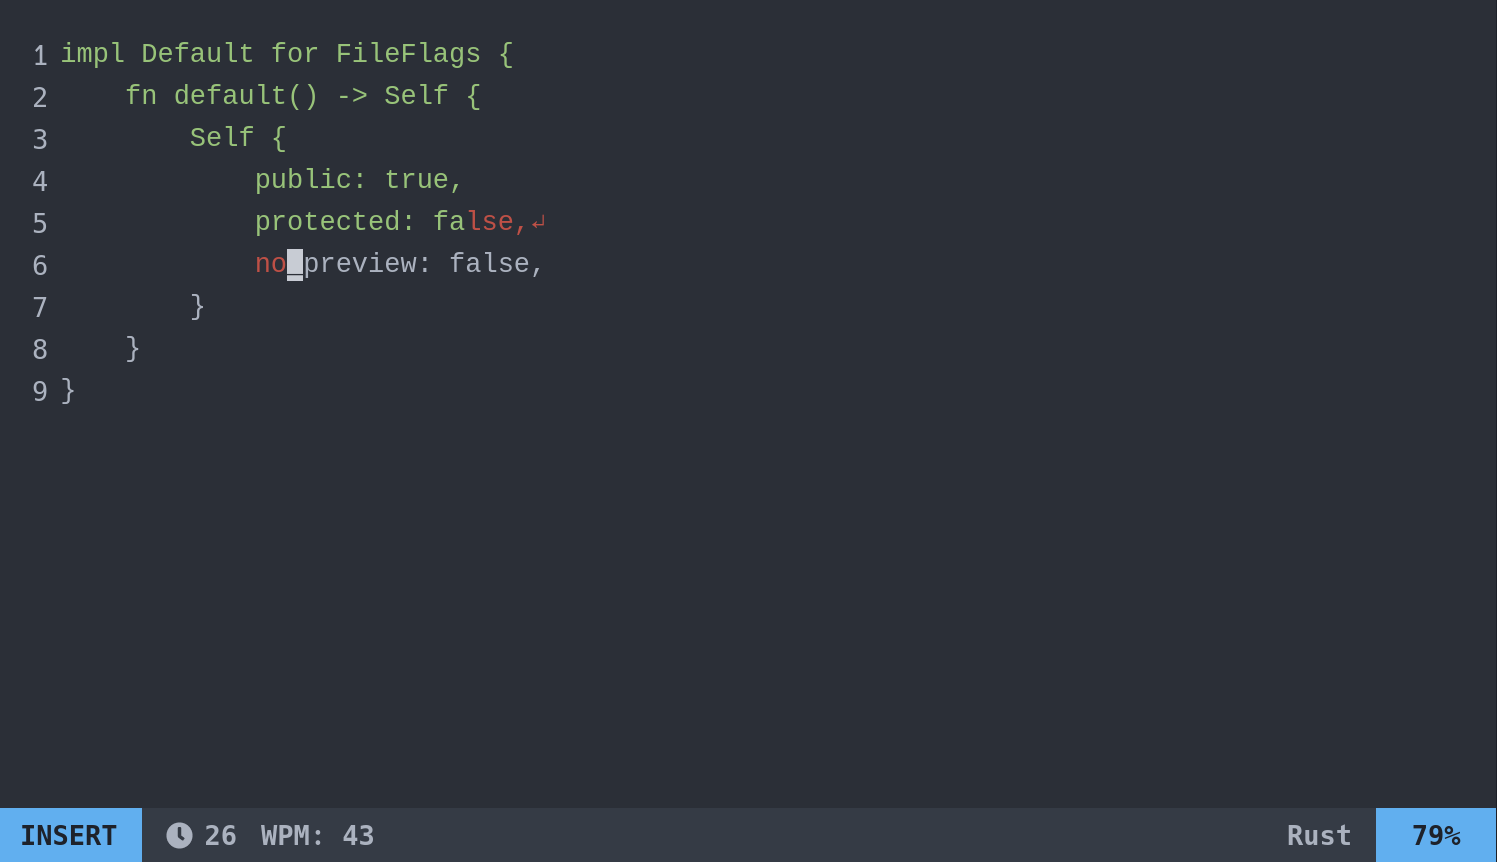
\includegraphics[width=\textwidth]{./figures/vim.png}
  \caption{typetest}
\end{figure}

Het is een simpele applicatie waarbij de gebruiker een willekeurig code fragment krijgt die hij zo
snel mogelijk moet overtypen. Tijdens het typen wordt er live, zijn tijd en woorden per minuut (WPM)
bijgehouden. Als de gebruiker het volledige fragment heeft overgetypt krijgt hij een resultaten
pagina te zien. Daar kan hij zijn statistieken bekijken zoals: WPM, verlopen tijd, accuraatheid en
het aantal fouten. Daarna kan de gebruiker opnieuw spelen door op de letter ‘r’ in te drukken. \\
\begin{wrapfigure}{l}{0.45\linewidth}
  \centering
  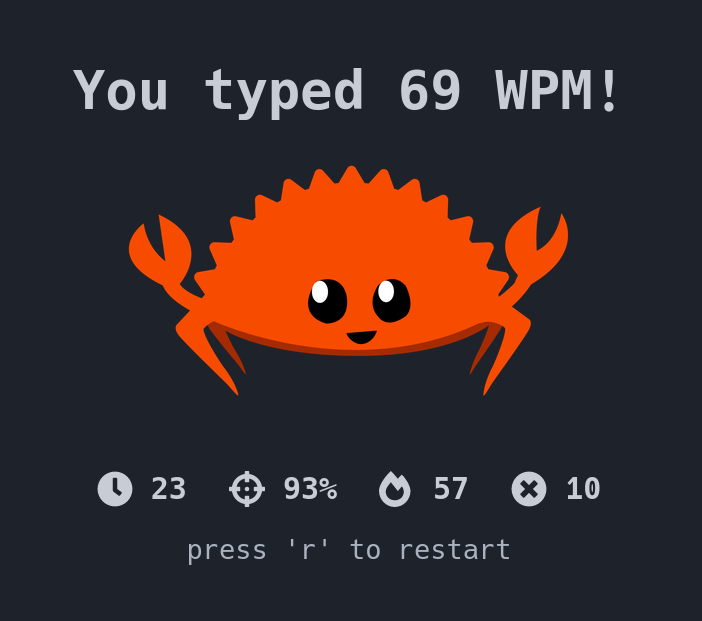
\includegraphics[width=\linewidth]{./figures/result.png}
  \caption{test resultaat}
\end{wrapfigure}


Er was voor ogen om bij dit project nog een aantal functionaliteiten eraan toe te voegen. Zoals
authenticatie met SSO, de statistieken opslaan in de database zodat er een lijn grafiek kon getoond
op basis van de historiek, andere database, profiel pagina, ci/cd enz. Helaas is het onderzoek niet
zo ver gekomen. Het leren van Rust en WebAssembly nam meer tijd in beslag dan verwacht. Zonder
voorkennis van Rust of een gelijkaardige systeem level programmeertaal was dit project al een hele
uitdaging op zich.

\clearpage

\section{Opbouw/structuur}

\begin{figure}[h]
  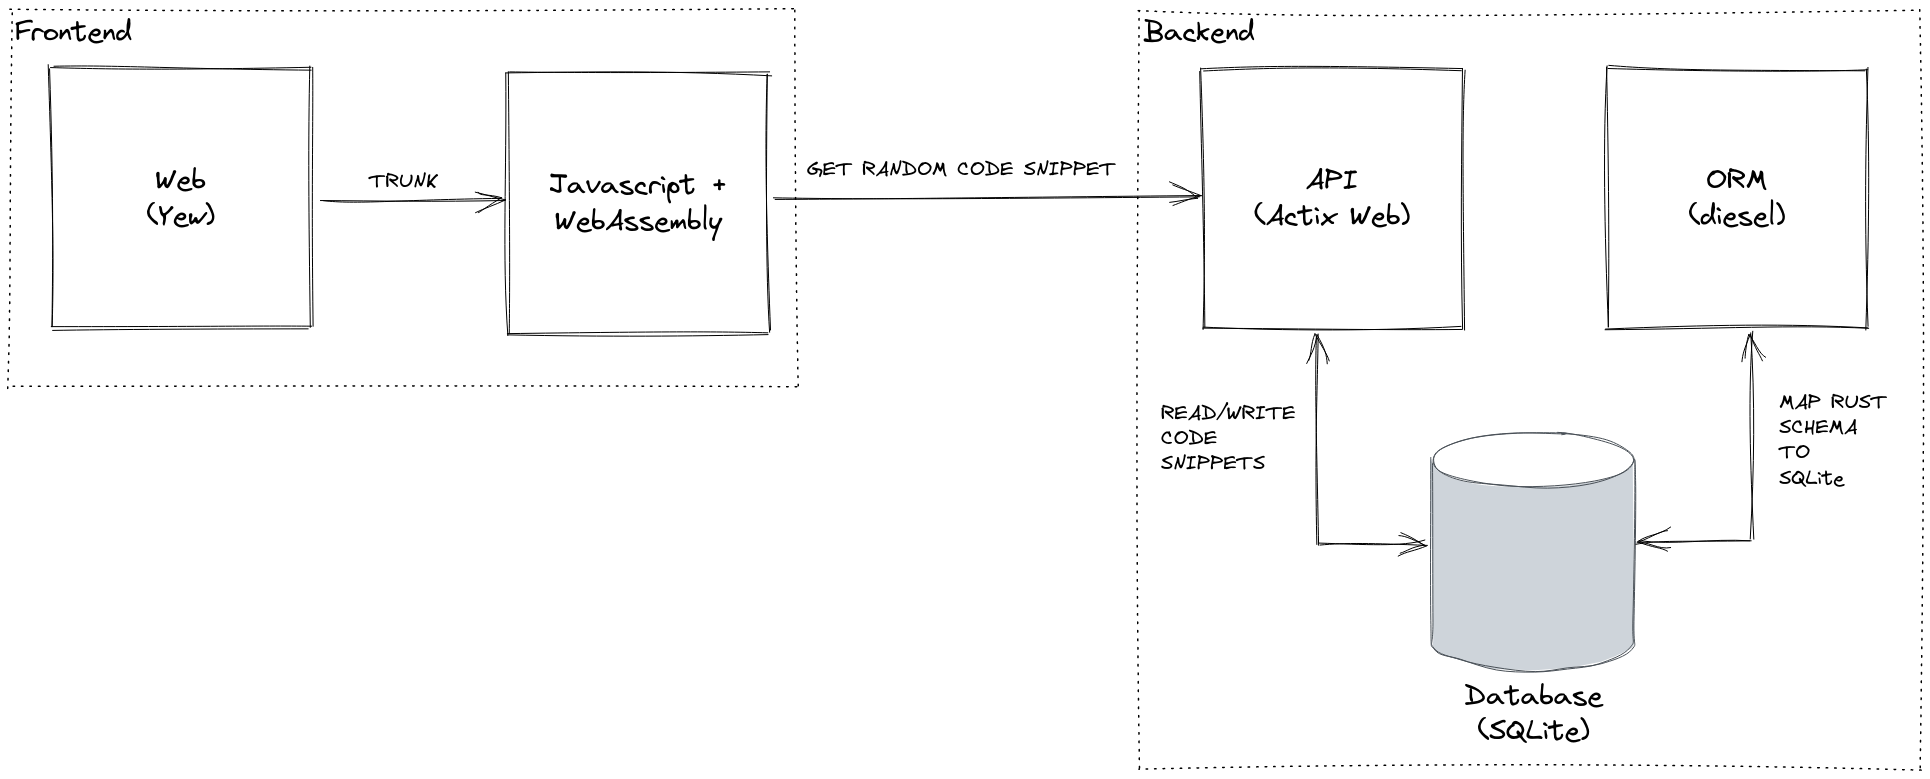
\includegraphics[width=\textwidth]{./figures/structuur.png}
  \caption{technisch schema}
\end{figure}

De frontend van de applicatie is volledig geschreven in Rust. Dit is mogelijk gemaakt door het
gebruik van Yew als framework. Daarbij is er Tailwindcss gebruikt als CSS framework. Tailwindcss is
een utility-first CSS framework om snel custom user interfaces te bouwen. Samen met een component
based framework als Yew hoeven we zelf geen CSS meer schrijven maar kunnen we direct tailwindcss
zijn utility classes toepassen op mijn components. Wat maakt voor een geweldige developer
experience. 

Om alles van frontend te kunnen compileren en uitvoeren is er trunk gebruikt. Trunk is een WASM web
applicatie bundelaar. Het gebruikt een eenvoudige config voor het bouwen en bundelen van WASM, JS
snippets en andere assets (images, css, scss) via een source HTML bestand. Met een simpel commando
als \mintinline{bash}{trunk build} bouwt hij de hele frontend en met \mintinline{bash}{trunk serve
--open} draait hij een lokale dev server.  

Bij het laden van de startpagina haalt de frontend een willekeurig code fragment op via de API. De
API haalt de fragmenten op uit een SQLite database. Om de database in sync te houden met de Rust
code werd er diesel gebruikt als ORM framework.


\clearpage

\section{Werking frontend}

De startpagina is geïnspireerd door mijn favoriete editor vim. Zo krijgt u een simpele versie van
vim te zien als editor voor het typen. Hieronder ziet u een schema van de compositie van de
belangrijkste components.

\begin{figure}[h]
  \centering
  
\includegraphics[width=0.9\textwidth]{./figures/components.png}
  \caption{structuur components}
\end{figure}

\mintinline{rust}{Game}: rendert op basis van de game status \mintinline{rust}{Vim} of
\mintinline{javascript}{Result} 

\mintinline{rust}{Vim}: de tekst editor voor de code en bevat \mintinline{rust}{Window} \&
\mintinline{rust}{StatusLine} als children 

\mintinline{rust}{Window}: rendert de tekst samen met \mintinline{rust}{LineNumber} 

\mintinline{rust}{StatusLine}: toont live statistieken zoals de huidige taal, tijd, WPM, progress 

\mintinline{javascript}{Result}: toont alle statistieken op het einde van de game

Het bouwen van de interface was redelijk eenvoudig, maar om de speed typing test te doen werken was
het verassend moeilijk. Het duurde enkele iteraties tot de logica goed zat. Om de gebruiker het idee
te geven dat hij tekst over typt zijn er vier html elementen gebruikt: een cursor met het huidige
karkater, de correct getypte tekst, de foute getypte tekst en de resterende tekst.

\begin{wrapfigure}{l}{0.55\textwidth}
  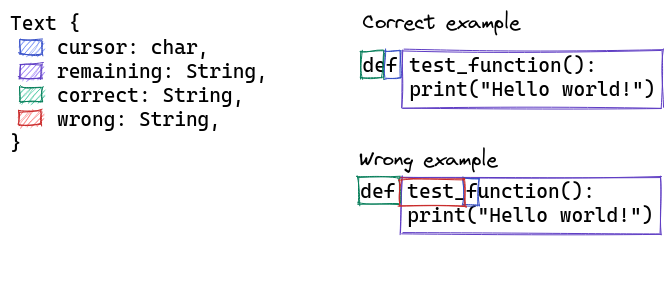
\includegraphics[width=\linewidth]{./figures/text.png}
  \caption{werking typen}
\end{wrapfigure}

Bij elk keypress event wordt er gecontroleerd of de key gelijk is aan het volgende karakter. Indien
het gelijk is wordt het huidige karakter van de cursor toegevoegd aan de string met de correcte
karakters en de cursor schuift een karakter op. Hetzelfde geldt als men een verkeerde key indrukt
maar de cursor wordt dan toegevoegd aan de string met de foutieve karakters. Als de gebruiker de
'Backspace' toets indrukt kan hij zijn foute karakters verwijderen tot de string leeg is. 

\clearpage

Dit was het basisidee, de moeilijkheid van het bouwen lag vooral aan hoe we efficiënt de variabelen
van de tekst en de bijhorende statistieken in een state kunnen opslaan zodat elk component slechts
rendert als het nodig is.  

Mijn eerste oplossing was het gebruik van globale state met de \mintinline{rust}{use_reducer} hook.
Als u vertrouwd bent met React zijn de meeste hooks zoals \mintinline{rust}{use_reducer},
\mintinline{rust}{use_state}, \mintinline{rust}{use_effect} overgenomen in Yew. Indien niet leg ik
het kort even uit. Om simpele variabelen op te slaan in een state zoals bijvoorbeeld een boolean
gebruikt u de \mintinline{rust}{use_state} hook. Die zorgt ervoor dat de boolean doorheen het
component lifecycle hetzelfde blijft tenzij u hem aanpast. Als u hem aanpast dan zal het component
opnieuw renderen.  

De \mintinline{rust}{use_reducer} hook werkt gelijkaardig maar wordt gebruikt voor complexere
states. Zo komt het met een dispatch functie die een argument neemt van het type Action. Wanneer
deze wordt aangeroepen, worden de actie en de huidige waarde doorgegeven aan de reducer functie die
een nieuwe state berekent en retourneert.

Zo heb ik 5 acties gedefinieert: \mintinline{rust}{NewSnippet}, \mintinline{rust}{Keypress},
\mintinline{rust}{Backspace}, \mintinline{rust}{Tick} en \mintinline{rust}{Reset}. In die acties zit
de meeste logica van het spel en kan gebruikt worden in components om de state van het spel aan te
passen. 

\begin{figure}[h]
\centering
\begin{minipage}{.45\textwidth}
\begin{minted}{rust}
pub struct Code {
  pub lines: usize,
  pub cursor: Option<char>,
  pub remaining: String,
  pub correct: String,
  pub wrong: String,
}

pub struct Stats {
  pub progress: u8,
  pub mistakes: u8,
  pub wpm: u8,
  pub accuracy: u8,
  pub time: u8,
  pub combos: u8,
}
\end{minted}
\end{minipage}%
\begin{minipage}{.45\textwidth}
\begin{minted}{rust}
pub struct GameState {
  pub code: Code,
  pub stats: Stats,
  pub status: Status,
  pub language: String,
}

pub enum Action {
  NewSnippet(Snippet),
  KeyPress(char),
  BackSpace,
  Tick,
  Reset,
}


\end{minted}
\end{minipage}
\end{figure}

Het probleem met de \mintinline{rust}{use_reducer} hook is dat een component de hele state opneemt.
Als de child components een variabel nodig hebben van de state, moeten die als properties worden
doorgeven. Hier is niks mis mee tenzij u een diep genest child component hebt die afhankelijk is
van de state. Dan heeft u 'prop drilling' waarbij u vanuit de parent component de props moet
doorgeven aan zijn children die dezelfde props dan doorgeven aan hun children, en zo verder tot dat
je bij de gewenste component bent.

\clearpage

\begin{figure}[h]
  \centering
  
\includegraphics[width=0.6\textwidth]{./figures/use_reducer.png}
  \caption{\mintinline{rust}{use_reducer}}
\end{figure}

Dit werd opgelost door de \mintinline{rust}{use_context} hook te gebruiken samen met de
\mintinline{rust}{use_reducer}. Zo kunnen we een \mintinline{rust}{GameStateProvider} component
definiëren die de context (state) consumeert en gebruikt kan worden door alle child components. Dit
betekent dat we de props niet meer hoefde te 'prop drillen' maar direct kon aanspreken vanuit alle
child components onder de \mintinline{rust}{GameStateProvider}. Helaas heeft deze methode ook zijn
nadelen: 
\begin{itemize}
    \item Als de state gebruikt wordt in een child component moet de hele state gekloond worden 

    \item Stel een child component gebruikt een variabele A van de globale state, als de hele state
    wordt aangepast behalve de variabele A zal het child component toch onnodig re-renderen 
\end{itemize}

Uiteindelijk is er de switch gemaakt naar yewdux, een state management library voor Yew die werkt
met een globale store/state. Het is verglijkbaar met de populaire React library Redux. Yewdux
gebruikt een CoW (clone on write) managementstrategie. Dit betekent dat de state bij elke mutatie
een keer wordt gekloond. Door het op deze manier te doen kunnen we beknopt een precieze mutatie
uitdrukken zonder extra boilerplate, en gebruik maken van change detection om onnodige re-renders te
voorkomen. 

Een voorbeeld hiervan is de \mintinline{rust}{use_selector} hook van yewdux, waarmee we een
variabele van de state kunnen selecteren en slechts re-renderen als de variabel verandert i.p.v. de
hele state.

\clearpage

\section{Werking backend}

De werking van de backend verschilt niet veel met het voorbeeld 'Todo' applicatie die we gemaakt
hebben in \enquote{Hoe bouwt u een API in Rust?}. Opnieuw werd er gekozen voor een simpele SQLite database
om de code snippets in op te slaan. Zoals eerder gezien wordt het database schema aangemaakt door
migrations uit te voeren met diesel CLI.  Dit is een database first aanpak, na wat onderzoek lijkt
het me dat diesel.rs jammer genoeg geen andere aanpakken ondersteund zoals code first. Met code
first kan u vanuit models die gedefinieerd staan in code automatisch migrations aanmaken die het
database schema aanpassen/aanmaken. 

In de speed typing database gebruiken we twee tabellen 'languages' en 'snippets'. Die een één op
veel relatie met elkaar hebben. De tabel languages bevat de soorten programmeertalen en de tabel
snippets de code. De code is hier gewoon opgeslagen als tekst in de tabel snippets. Het is wel
belangrijk dat de code geen spaties bevat maar tabs. Daarvoor is er kleine parser tool geschreven om
makkelijk code snippets te maken. Het neemt een tekstbestand als input en zet alle spaties en enters
om naar de respectievelijke karakters '\textbackslash t' en '\textbackslash n'. Zo kan de frontend
makkelijk de juiste enters en tabs weergeven. 

De API kent een aantal routes:
\begin{itemize}
    \item GET, POST, DELETE  /languages
    \item GET, POST, DELETE /snippets 
    \item GET /snippets/random 
    \item GET /snippets/\{language\_id\}
\end{itemize}

Uiteindelijk gebruikt de frontend maar een route '/snippets/random' om een willekeurig code fragment
op te halen uit de database. 

Om ervoor te zorgen dat we niet eerst alle fragmenten op halen uit de database om dan een willekeurig
fragment eruit te selecteren. Wordt er eerst via een SQL-query de snippets tabel willekeurig gesorteerd
en het eerste resultaat eruit gepakt. Standaard zal Rust of diesel het random type niet kennen.
Gelukkig voorziet diesel de \mintinline{rust}{no_arg_sql_function} macro waarmee u SQL functies kunt
mappen naar Rust types.

\begin{listing}[h]
\begin{minted}{rust}
no_arg_sql_function!(
  random,
  sql::types::Integer,
  "Represents the SQL RANDOM() function"
)
\end{minted}
\end{listing}

Zo kunnen we het random type importeren vanuit het schema en gebruiken in mijn SQL-query opgesteld
door diesel.
